\documentclass[../TST.tex]{subfiles}
\begin{document}
\begin{eproblem}[Efficiency of a circuit]{\ \\[5pt]}
\textit{Equipment:}\\
DC voltage source (rectifier), 3 multimeters, resistor substitution box $R_x$, two resistors $R_1$ and $R_2$ in series, 8 wires, graph paper. See Figure \ref{fig3}.\\

\begin{figure}[h]
\centering
% \hspace*{0.6cm}
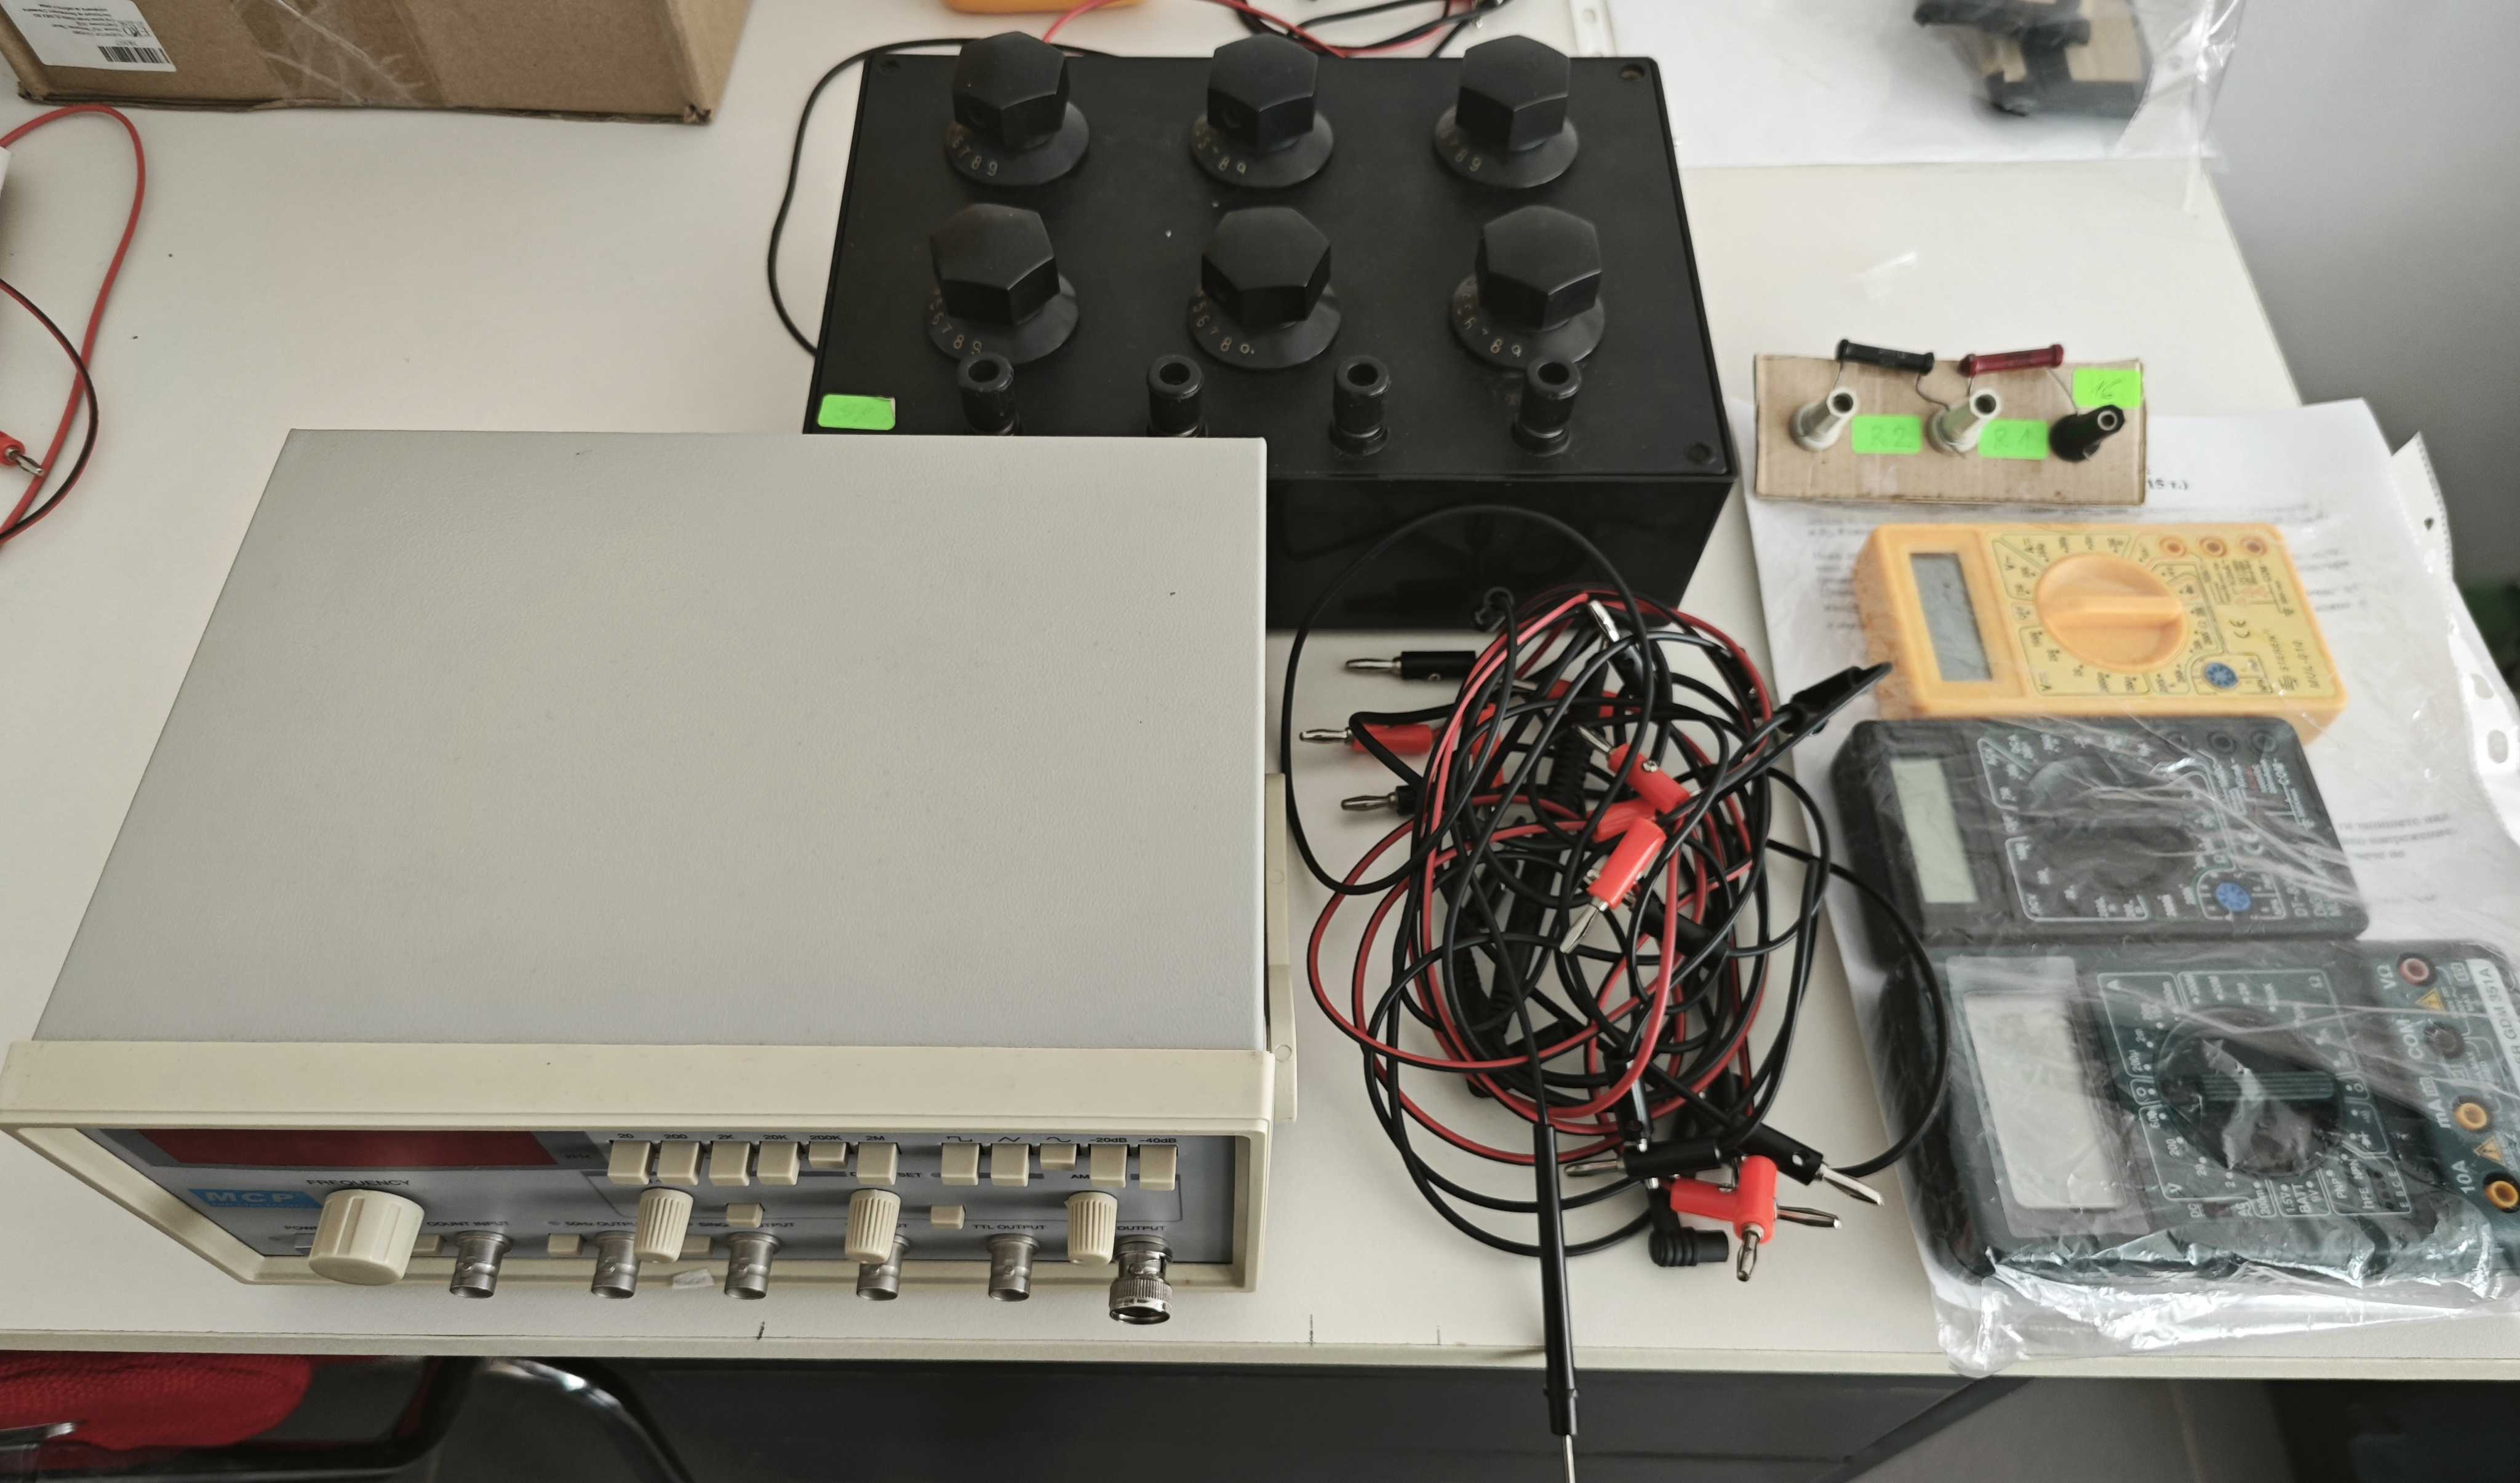
\includegraphics[width=0.8\textwidth]{fig/2015_e1.jpg}
\caption{}
\label{fig3}
\end{figure}

Let us define the efficiency of the circuit on Figure \ref{fig4} as the ratio of the power dissipated to the right of the voltmeter (i.e. at the resistor $R_x$ and the ammeter $I_x$) to the total power dissipated in the circuit. The aim of this problem is to study the dependence of $\eta$ on the load $R_x$ (which will be calculated as $R_x=U_x/I_x$). This will be used to find the optimal value $R_{x,\mathrm{opt}}$ which maximises $\eta$ (accurate to $\qty{5}{\ohm}$), as well as the maximum $\eta$ itself. 
\begin{figure}[h]
\centering
% \hspace*{0.6cm}
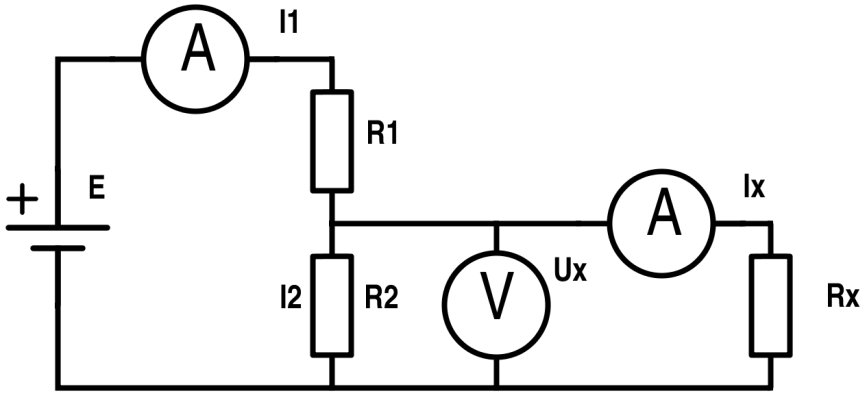
\includegraphics[width=0.6\textwidth]{fig/2015_l2.png}
\caption{}
\label{fig4}
\end{figure}

\begin{subpart}
	\item Using a multimeter in ohmmeter mode, measure the resistances $R_1$ and $R_2$ and record them in a table. Turn on the voltage source in DC mode and set the voltage to $E=\qty{2.00}{V}$. Leave the source on and do not change the voltage from now on. \score{1.0} 
	\item Assemble the circuit. Before connecting it to the voltage source, ask the examiner to confirm. \score{3.0}
	\item Assume that the dependence $\eta(R_x)$ has a single maximum. Choose appropriate values for $R_x$ in the range ($0.1R_x$ -- $10R_x$). Take the necessary measurements and tabulate the dependence for this range. In the table you should record both the nominal resistance of the substitution box and its measured value $R_x=U_x/I_x$. \score{5.0}
	\item Plot a graph of $\eta(R_x)$. \score{2.0}
	\item If your experimental data is insufficient, take additional measurements. If the scale of your graph was unsuitable, plot an additional graph which covers only the important features of the dependence. Write down your values for $R_{x,\mathrm{opt}}$ and $\eta(R_{x,\mathrm{opt}})$. \score{4.0}
\end{subpart}
Call the examiner in case of any technical difficulties.\\
\end{eproblem}
\end{document}
